\chapter{Desenvolvimento}
\section{Hardware}
\subsection{TIVA e seus pontos fracos}
O desenvolvimento foi iniciado com a placa EK-TM4C1294XL, que contém o controlador TM4C1294NCPDT. 
Embora a placa possua capacidade 

\color{orange}
Placa EK-TM4C1294XL que contém o controlador TM4C1294NCPDT

Não possui firmware específico para essa aplicação (recepção e reprodução de áudio)

Não possui I2S

I2S pode ser emulado com dois I2C, porém apresenta dificuldades com outros componentes da placa

Software próprio se tornou instável a ponto de impedir o desenvolvimento

Precisaria de uma placa com componentes próprios (codec, DAC, Conector P2) para serem iniciados os testes
\subsection{STM32F769I-DISCO e suas vantagens}

Já possui firmware base para comunicação USB

Possui saída de áudio e display LCD com touch; facilita protótipos

Possui I2S, sendo possível seu uso nativo

Controlador STM32F769NI possui capacidade um pouco maior de processamento 
\color{black}

\subsection{Possíveis hosts para o device}

Diversos sistemas operacionais possuem as especificações necessárias para se comunicarem com o dispositivo sem necessidade de instalação de drivers. Os sistemas mais utilizados em computadores pessoais atualmente, como Windows, Linux e MacOS, possuem drivers para comunicação com dispositivos de áudio por USB.

Além disso, sistemas operacionais de dispositivos móveis também possuem compatibilidade direta com o dispositivo. Nessa lista, incluem-se os dois sistemas mais utilizados, Android e iOS.

Embora os computadores ou dispositivos móveis nos quais os sistemas operacionais estão inseridos possivelmente já possuam uma solução de saída de áudio, é possível ser feita a sobreposição desse sistema, onde o áudio é enviado ao dispositivo ao invés de pela saída padrão.

\begin{figure}[!h]
  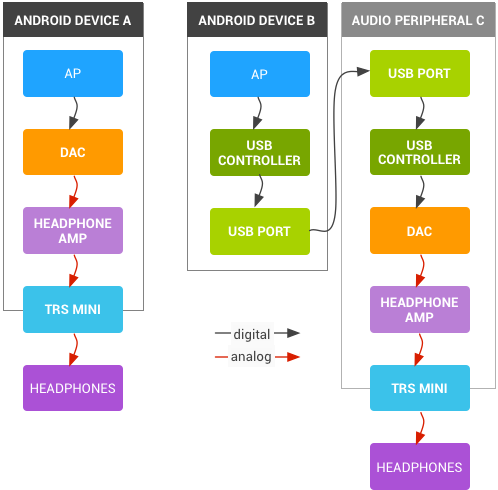
\includegraphics[scale=0.5]{figuras/usb-android-dscs.png}
  \caption{!! TROCAR POR VERSÃO DE AUTORIA PRÓPRIA !!}
  \label{fig:synchronousMode}
\end{figure}


\subsection{Componentes}

\subsubsection{Serial Audio Interface Codec}
% https://www.st.com/resource/en/product_training/STM32F7_Peripheral_SAI.pdf

\color{red}
An audio codec with four DACs and two ADCs is connected to the SAI interface of the
STM32F769NIH6. It communicates with the STM32F769NIH6 via an I2C bus shared with
the touch panel of the LCD DSI:
• The analog line input is connected to the ADC of the codec device via an audio jack
(CN6).
• The analog line output is connected to the DAC of the codec device via an audio jack
(CN7).
• Two external speakers can be connected to the codec device via the JP2 for the left
speaker and JP3 for the right speaker.
• Four digital microphones (ST MEMS microphone) are available on the
32F769IDISCOVERY Discovery board. They are connected to the input digital
microphones of the STM32F769NIH6 and the DFSDM functionality manages them.
• One coaxial connector (CN12) is implemented on the 32F769IDISCOVERY to receive
external audio data compatible with SPDIF specifications.
• One coaxial connector (CN8) is implemented on the 32F769IDISCOVERY to output
external audio data compatible with SPDIF specifications.

For audio playback, the STM32 board is recognized by the PC (USB Host) as a USB
speaker. The PC sends audio samples to the board via the USB. The STM32 MCU
configures the audio codec via the I2C
% https://www.cirrus.com/products/wm8994/
The WM8994 is a highly integrated, ultra low power hi-fi codec with an integrated stereo Class D and AB speaker driver, and a Class W headphone driver to minimize power consumption during audio playback. The device requires only Vbatt and a 1.8V supply, generating all other internal supply rails from integrated LDOs. Stereo full duplex asynchronous sample rate conversion and multi-channel digital mixing combined with powerful analog mixing to support a wide range of different architectures and use cases. A fully programmable parametric EQ provides speaker compensation and a dynamic range controller can be used in the ADC or DAC paths for maintaining a constant signal level, maximizing loudness and protecting speakers against overloading and clipping. A smart digital microphone interface provides power regulation, a low jitter clock output and decimation filters for up to four digital microphones. A MIC activity detect with interrupt is available. Active ground loop noise rejection and DC offset correction help prevent pop noise and suppress ground noise on the headphone outputs.
\color{black}

\color{orange}
Possui DAC de 24bits e 4 canais

Driver de 2W classe D/AB
\color{black}

\subsubsection{Output Jack}

\section{Firmware}

\subsection{Inicialização de projeto}

Existem diversas maneiras de se iniciar um projeto para placas da STM, cada um focando em uma ponta do ecosistema criado pela empresa.

Projetos podem ser criados pelo Mbed Studio, que possui uma interface mais moderna baseada no VSCode (o editor com maior crescimento entre desenvolvedores nos últimos anos), e se propôe a facilitar o ponto de entrada para desenvolvimento e encurtar o processo desde concepção até funcionamento. Para atingir essa proposta, porém, esta IDE acaba sendo mais limitada em questão de controle fino do hardware, tornando-se dependente de bibliotecas já prontas ou que façam ponte com o editor para que o usuário possa acessar a funcionalidade desejada.

Outro caminho para a criação dos projetos conta com a utilização do STM32CubeIDE, uma IDE baseada no mais tradicional editor Eclipse. Embora possua uma experiência de usuário mais defasada em relação ao editor anterior, funcionalidades de controle gráfico do hardware e de configurações das funcionalidades da placa oferecem um maior controle sem uma grande diminuição da produtividade. Essas funcionalidades se tornam possíveis devido à geração automática de código disponibilizada pelo editor. Alterações em parâmetros, ou ativação/desativação de funcionalidades da placa desencadeiam mudanças automáticas de código, configurando inicializações, registradores e outros processos necessários de maneira automatizada.

\begin{figure}[!h]
  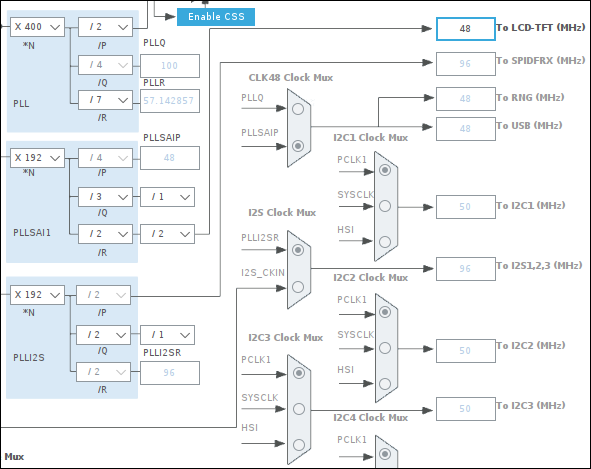
\includegraphics[scale=0.5]{figuras/clock.png}
  \caption{Exemplo de configuração visual de parâmetros de clock disponibilizado pela STM32CubeIDE}
  \label{fig:visualClockEdit}
\end{figure}


Anterior à disponibilidade do STM32CubeIDE, projetos tipicamente eram criados com a ferramenta SW4STM32, proveniente de uma empresa terceira, também baseada em Eclipse. Diversos projetos estruturados com a intenção de demonstrar a construção inicial para diversas funcionalidades (como a transmissão de áudio utilizando as camadas de abstração de hardware disponíveis) foram criadas nesse formato. Embora o uso dessa IDE seja deprecada atualmente, seus projetos podem ser convertidos para o foramto do STM32CubeIDE, embora com perdas de algumas de suas funcionalidades (como a edição visual de parâmetros das funcionalidades da placa). Isso se dá devido a conflitos entre o código automaticamente gerado pela IDE e o código legado já presente no projeto.

Para este projeto, foi utilizado um projeto de áudio base iniciado em SW4STM32, e migrado para STM32CubeIDE. 

\color{orange}
Essa escolha foi tomada pensando na melhor relação entre o ganho de produtividade com a utilização de ferramentas mais avançadas, o ganho de produtividade presente em utilizar uma base já pré-configurada de comunicação USB, e a facilidade de utilização das ferramentas.
\color{black}


\subsection{HAL, BSP e CMSIS}
Este projeto conta utiliza a arquitetura de abstração de hardware necessária para desenvolvimento de hardware em controladores da STM32. 

A arquitetura principal pode ser dividida em três níveis:
\begin{itemize}
    \item Nível 2: Aplicação. Essa camada contém a lógica de mais alto nível que tem como função implementar as funcionalidades da aplicação em si. O código desenvolvido pelo usuário dos microcontroladores costuma ficar em grande parte nessa camada, indo para camadas de mais baixo nível conforme necessário. Nessa camada também podem ser encontrados projetos de exemplo de utilização da placa (como demonstrações básicas de relações entere botões e LEDs, por exemplo), e projetos de código padronizado que montam uma base para que um projeto possa ser feito em cima dele.

    \item Nível 1: \textit{Middleware}. Nessa camada são encontradas bibliotecas de código que tem como função realizar a interface entre as camadas de mais baixo nível de abstração e a camada de aplicação. Um exemplo de middleware é o FreeRTOS, um sistema operacional em tempo real que permite a utilização de conceitos de execução de tarefas em pseudo paralelismo com restrições de tempo de execução.

    \item Nível 0: Drivers. Esse nível se divide em diversas bibliotecas que tem como intuito realizar a interface direta entre o hardware e as camadas de mais alto nível. APIs para inicialização, configuração e comunicação com periféricos como I2C e UART. Entre as bibliotecas encontradas nessa camada, estão a HAL (Hardware Abstraction Layer), BSP (Board Support Package) e CMSIS (Common Microcontroller Software Interface Standard).
\end{itemize}


% https://en.wikipedia.org/wiki/Hardware_abstraction
% https://www.techopedia.com/definition/4288/hardware-abstraction-layer-hal
% https://emteria.com/learn/hardware-abstraction-layer
\begin{figure}[!h]
  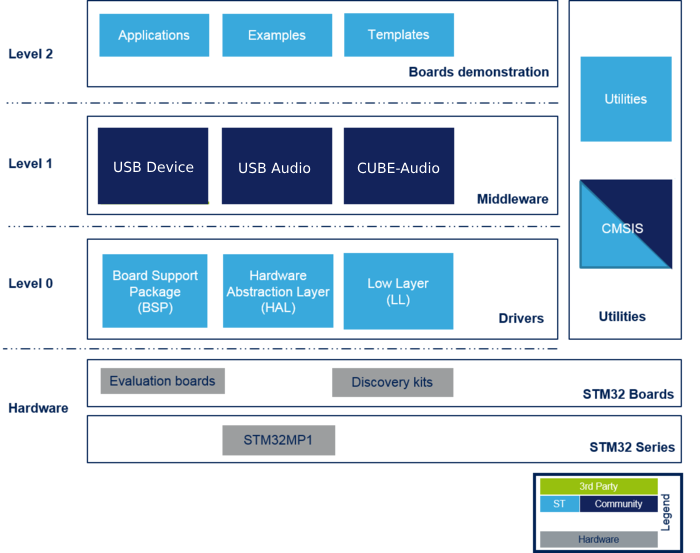
\includegraphics[scale=0.5]{figuras/stm32-architecture.png}
  \caption{Desenho de arquitetura do ecossistema STM32 embarcado !! marcar como adaptado !!}
\end{figure}

A \textit{Hardware Abstraction Layer (HAL)} é uma biblioteca de código que possui a função de entregar uma interface de desenvolvimento padronizada que permita interações com o hardware sem necessidade do conhecimento direto do hardware em questão. Essa biblioteca tem seu foco na comunicação com periféricos internos, como os de acesso direto de memória (DMA) e de interface serial de áudio (SAI).
% [[FONTE]](https://emteria.com/learn/hardware-abstraction-layer).

Isso permite uma maior portabilidade do código, o qual se torna compatível com qualquer hardware que também esteja incluso nessa camada de abstração.
Uma HAL é comumente utilizada para realização do trabalho de inicialização, configuração e acesso a um hardware específico. Para este projeto, foi utilizada a HAL V1.2.6, lançada em 29 de junho de 2018.
\\[10pt]

A \textit{Board Support Package (BSP)} é uma coleção de APIs, drivers e arquivos de configuração que tem como intuito facilitar o desenvolvimento em uma placa específica. Sua composição é geralmente feita em interface com APIs da Hardware Abstraction Layer (HAL), com a intenção de sintetizar uma API ainda de mais fácil utilização para o hardware conhecido de uma determinada placa.

Para este projeto, foi utilizado a BSP da placa STM32F769I-DISCO.
\\[10pt]

O \textit{Common Microcontroller Software Interface Standard (CMSIS)}, é um conjunto de bibliotecas que implementam funcionalidades comumente utilizadas no desenvolvimento embarcado, com o intuito de reduzir o atrito inicial do desenvolvimento, evitar re-trabalhos e reduzir e o tempo até o mercado de um produto até o mercado. Ele funciona em paralelo à Hardware Abstraction Layer, inclusive dependendo da versão específica dessa abstração para alguma de suas funcionalidades. Diferentemente da HAL e BSP, esta biblioteca não é diretamente ligada à STM32, e sim compartilhada entre diversas empresas que possuem seus controladores desenvolvidos na tecnologia ARM.


Embora as bibliotecas BSP e HAL sejam criadas pela STM32, sua compatibilidade não é imediatamente garantida. Para seu funcionamento correto, as bibliotecas devem estar em versões compatíveis entre si.

No projeto \textit{X-CUBE-USB-AUDIO}, disponibilizado pela STM32 como exemplo de comunicação os periféricos de áudio por meio das bibliotecas de abstração, uma versão mais antiga da HAL foi utilizada como base para a interface entre o nível de aplicação e os periféricos de USB e áudio. Este projeto possui como base a versão 1.2.6 da HAL, disponibilizada em junho de 2018. Novos projetos criados pela IDE STM32CubeMX, porém, contam por padrão com a versão mais nova (que, durante o desenvolvimento deste projeto, era a versão 2.0.2, de junho de 2022).

As duas versões utilizadas da HAL possuem diferenças suficientes entre si a ponto de serem incompatíveis. Embora possuam essencialmente a mesma funcionalidade (com correções de problemas e otimizações presentes na versão mais nova), mudanças em parâmetros de funções e estruturas de dados, como mostrado na Listagem \ref{code:hal-differences}, não permitem que um código escrito para uma versão antiga da HAL seja integrado a um código escrito para a versão mais recente.

\begin{sourcecode}[!ht]
\centering
\begin{minted}{c}
// v1.2.6
typedef struct
{
    int8_t  (*Init) (
        USBD_AUDIO_FunctionDescriptionfTypeDef* as_desc, 
        uint32_t private_data
    );
    int8_t  (*DeInit) (
        USBD_AUDIO_FunctionDescriptionfTypeDef* as_desc,
        uint32_t private_data
    );
    int8_t  (*GetConfigDesc) (
        uint8_t **p_data, 
        uint16_t *p_size, 
        uint32_t private_data
    );
    int8_t  (*GetState) (uint32_t privatedata);
    uint32_t private_data;  
} USBD_AUDIO_ItfTypeDef;


// v2.0.2
typedef struct
{
  int8_t (*Init)(uint32_t AudioFreq, uint32_t Volume, uint32_t options);
  int8_t (*DeInit)(uint32_t options);
  int8_t (*AudioCmd)(uint8_t *pbuf, uint32_t size, uint8_t cmd);
  int8_t (*VolumeCtl)(uint8_t vol);
  int8_t (*MuteCtl)(uint8_t cmd);
  int8_t (*PeriodicTC)(uint8_t *pbuf, uint32_t size, uint8_t cmd);
  int8_t (*GetState)(void);
} USBD_AUDIO_ItfTypeDef;

\end{minted}
\caption{Exemplo de diferença de uma mesma estrutura de dados em diferentes versões da Hardware Abstraction Layer (HAL)}
\label{code:hal-differences}
\end{sourcecode}

Com o intuito de se utilizar a versão mais nova da HAL, foi tomado como foco de desenvolvimento a atualização do projeto de áudio para a versão mais nova da biblioteca, a fim de tornar o projeto compatível com as versões mais recentes geradas pela IDE.

Esta atualização se tornou inviável, porém, devido à integração também existente entre a biblioteca de suporte de placa (BSP) e a HAL. Como a BSP tem como função trazer uma abstração focada em componentes específicos de uma placa de desenvolvimento, muitas vezes chamadas de APIs da HAL são utilizadas (já que várias placas utilizam controladores idênticos ou similares, com muitos periféricos em comum). Isso implica que a atualização da HAL em um projeto faz com que chamadas da BSP parem de funcionar, devido a esperarem uma versão específica ao realizarem chamadas para a HAL. Em diversas situações, essas incompatibilidades se demonstravam apenas como \textit{hard faults}, devido a acessos indevidos de memória.

Para que o projeto de áudio ficasse compatível com novos projetos, uma re-escrita extensiva de diversos módulos de ambas BSP e HAL seria necessária. Uma avaliação foi então feita da complexidade das chamadas de periféricos que seriam utilizados na versão moderna da HAL (como comunicações serial, com a tela LCD e sua interface \textit{touch}). Como esses periféricos não são utilizados tão a fundo quanto a sequência de periféricos USB e de saída de áudio, foi constatado que o processo inverso, de rebaixar a versão da HAL utilizada pelos periféricos no projeto mais atualizado, seria mais produtivo.

Essa abordagem, embora também perdendo facilidades como a configuração visual de componentes disponibilizada para projetos mais modernos, ainda se mostrou mais viável, e permitiu a utilização simultânea de todos os periféricos necessários para o funcionamento do projeto.
\color{orange}


% Horoscope: V1.2.6 / 29-June-2018
% ApplePie: V2.0.2 / 10-June-2022

% // v1.2.6
% typedef struct
% {
%     int8_t  (*Init)         (USBD_AUDIO_FunctionDescriptionfTypeDef* as_desc , uint32_t private_data);
%     int8_t  (*DeInit)       (USBD_AUDIO_FunctionDescriptionfTypeDef* as_desc,uint32_t private_data);
%     int8_t  (*GetConfigDesc) (uint8_t ** p_data, uint16_t * p_size, uint32_t private_data);
%     int8_t  (*GetState)     (uint32_t privatedata);
%     uint32_t private_data;  
% } USBD_AUDIO_ItfTypeDef;


% // v2.0.2
% typedef struct
% {
%   int8_t (*Init)(uint32_t AudioFreq, uint32_t Volume, uint32_t options);
%   int8_t (*DeInit)(uint32_t options);
%   int8_t (*AudioCmd)(uint8_t *pbuf, uint32_t size, uint8_t cmd);
%   int8_t (*VolumeCtl)(uint8_t vol);
%   int8_t (*MuteCtl)(uint8_t cmd);
%   int8_t (*PeriodicTC)(uint8_t *pbuf, uint32_t size, uint8_t cmd);
%   int8_t (*GetState)(void);
% } USBD_AUDIO_ItfTypeDef;

% STM32CubeF7 Firmware Package V1.17.0 / 10-June-2022



% https://wiki.st.com/stm32mpu/index.php?title=STM32CubeMP1_architecture&oldid=77377
% As partes não são diretamente compatíveis: BSP, HAL e CMSIS devem estar em versões corretas para que sua interação ocorra corretamente

% A versão de BSP utilizada no projeto base de comunicação de áudio USB utilizava uma versão antiga da HAL

% As bibliotecas de interface humana (\textit{display}, \textit{touch}, serial) utilizavam uma versão mais atualizada da HAL

% A ideia inicial era de portar o código antigo da BSP de áudio USB para a nova HAL (e permitir a utilização das funcionalidades de controle visual de hardware)

% A junção inicial dos códigos não foi bem sucedida, fazendo com que as funcionalidades em conjunto causassem hard faults sem motivo aparente

% A causa eram devido a mudanças entre versões da HAL serem bem abrangentes, incluindo parâmetros de funções e estruturas de dados

% Foram identificados problemas onde acessos indevidos de memória devido à mudança das estruturas (onde uma estrutura era acessada no formato de outra estrutura, causando undefined behavior

% Atualizar a versão antiga da BSP precisaria quase de uma reescrita do código de conexão com a HAL, o que incluiria re-escrita de toda a camada de abstração de comunicação USB

% Foi preferido realizar o processo inverso, e realizar um \textit{downgrade} da HAL das funcionalidades de interface humana para serem compatíveis com o código BSP de áudio USB

Outra causa de \textit{hard faults} era devido a os códigos eram inicializados simultaneamente. Cada módulo funcionava corretamente em isolamento, porém causavam a placa a parar de responder caso fossem inicializados juntos

Além do problema inicial de diferença estrutural, foi identificado que um problema de timing ocorria entre as bibliotecas, onde alguns registradores eram acessados ou escritos em momentos que estavam sendo acessados por outra biblioteca. A adição de um atraso entre as inicializações das diferentes funcionalidades deixou a inicialização da placa um pouco mais lenta, porém resolveu completamente o problema de \textit{hard faults} no momento de inicialização
\color{black}

% [https://www.arm.com/technologies/cmsis#:~:text=Common Microcontroller Software Interface Standard,to market for new devices](https://www.arm.com/technologies/cmsis#:~:text=Common%20Microcontroller%20Software%20Interface%20Standard,to%20market%20for%20new%20devices).

% https://deepbluembedded.com/stm32-hal-library-tutorial-examples/

% https://www.st.com/resource/en/product_training/STM32G0-Ecosystem-STM32Cube-G0-Firmware-Package.pdf

% https://arm-software.github.io/CMSIS_5/General/html/index.html

\subsection{Configuração como dispositivo de áudio USB}
Algumas configurações precisam ser enviadas na conexão com a fonte para que o dispositivo seja reconhecido corretamente como um dispositivo de áudio. Duas das principais configurações necessárias são os VIDs e PIDs, ambos números de 16 bits tipicamente representados em hexadecimal.

\subsection{Seleção de parâmetros para transmissão}
\color{orange}
Explicar por que foi escolhido 48k (comentar das poucas diferenças em taxas maiores de amostragem e até problemas de fold back/fold over


Comentar do uso de 2 canais (stereo)

Comentar do uso de 16 bit (mostrar relação com noise floor já aceitável)

Comentar de buffer size ser 10240 bytes (com margem de 1 packet)



% // computes the nominal size(number of bytes) of an audio packet required for one millisecond
% // e.g. for 48KHZ   / 24 bits / stereo, the required size is 48 * 3 * 2
% //      for 44.1KHZ / 16 bits / stereo, the required size is 44 * 2 * 2
% #define AUDIO_MS_PACKET_SIZE(freq,channel_count,res_byte) (((uint32_t)((freq) /1000)) * (channel_count) * (res_byte)) 

% // computes the maximum size(number of bytes) of an audio packet required for one millisecond(without computing the sample added for synchronization)
% // e.g. for 48KHZ   / 24 bits / stereo, required size is 48 * 3 * 2
% //      for 44.1KHZ / 16 bits  /stereo, required size is 45 * 2 * 2
% #define AUDIO_MS_MAX_PACKET_SIZE(freq,channel_count,res_byte) AUDIO_MS_PACKET_SIZE(freq+999,channel_count,res_byte)

Packet para 1ms em 48KHz e 16 bits stereo contém 48 * (16 / 8) * 2 = 192bytes
\color{black}

% https://en.wikipedia.org/wiki/USB_Implementers_Forum

\subsection{Identificação como dispositivo de áudio por dispositivos host}

\textit{VIDs (Vendor IDs)} são números que identificam um fabricante ou fornecedor de dispositivos USB. Esse identificador é fornecido pelo USB Implementers Forum, necessitando de licenças anuais de custo elevado. Algumas fabricantes de microcontroladores permitem o uso de sua licença para fins não comerciais ou de pequena escala. Este projeto utiliza o vendor ID da STMicroelectronics (0x0483)

\textit{PIDs (Product IDs)} são números que identificam o dispositivo de maneira diferente para o sistema operacional ao qual ele está se conectando. Esse identificador varia de acordo com cada fornecedor.

Para esse dispositivo ser reconhecido como uma saída de áudio da STMicroelectronics, ele precisa informar ao sistema operacional que está se conectando o identificador 0x5730.

\subsection{Armazenamento (buffer circular)}
Como o modo de tranferência não possui correção de erro nem bufferização de dados, precisamos utilizar de um armazenamento temporário para podermos manipular e enviar o dado para frente.
\begin{figure}[!h]
  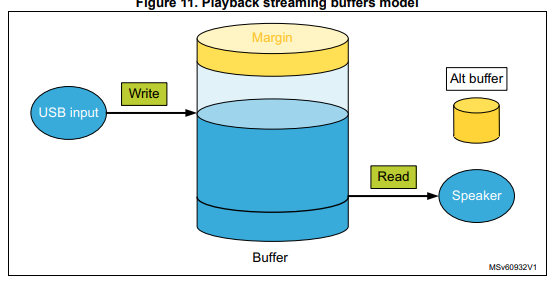
\includegraphics[scale=0.5]{figuras/circular-buffer.png}
  \caption{!! TROCAR POR VERSÃO DE AUTORIA PRÓPRIA !!}
  \label{fig:circularBuffer}
\end{figure}

Para se adequar ao padrão produtor-consumidor utilizado na transmissão USB, um buffer circular é utilizado. 

Ponteiros de leitura e escrita são utilizados para indicação de onde novos pacotes devem ser lidos e onde devem ser escritos, respectivamente. O ponteiro de leitura é administrado pelo nó de saída de áudio, e o de escrita pelo nó de entrada USB.

\begin{figure}[!h]
  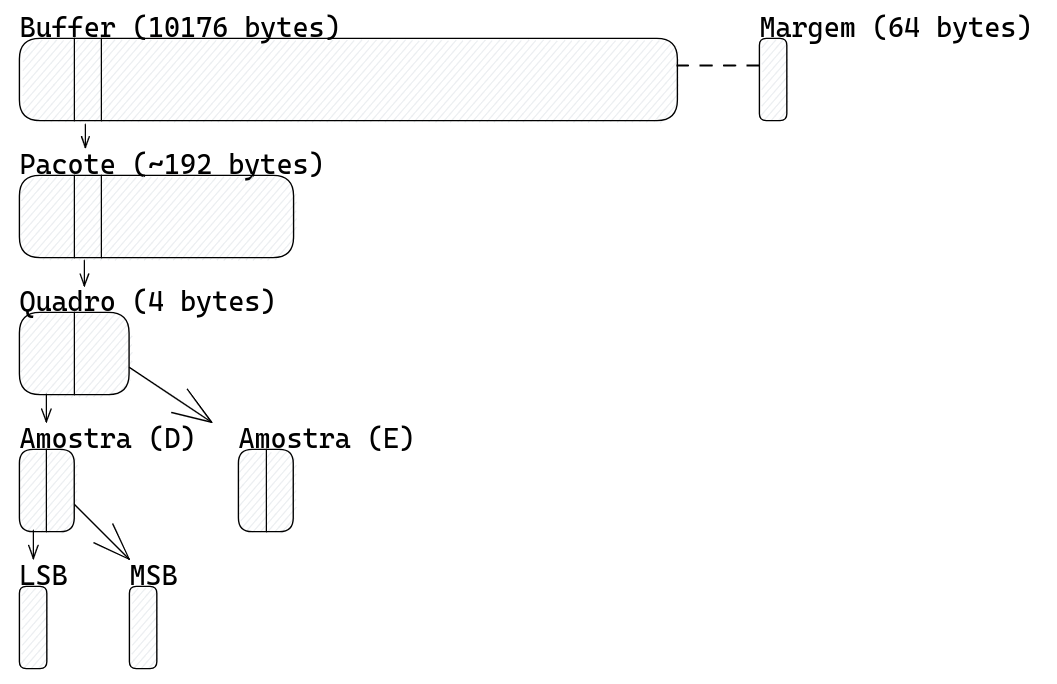
\includegraphics[scale=0.4]{figuras/buffer.png}
  \caption{Representação das partes que compõem o buffer circular}
  \label{fig:bufferBytes}
\end{figure}

\color{orange}

Explicar como dados são inseridos no buffer. O ponteiro de escrita é então incrementado para refletir a presença dos novos dados presentes no buffer.

Explicar como dados são consumidos do buffer. O ponteiro de leitura é incrementado para refletir esta leitura.
\color{black}

Através de DMA, os dados são então transferidos para o SAI (e em sequência para o codec).

Para todas as escritas e leituras serem de uma área contínua de memória, uma margem é adicionada ao *buffer*. Isso permite que dados sejam escritos de maneira contínua, mesmo caso o ponteiro de escrita esteja próximo do fim do buffer.

Caso dados sejam escritos de forma que ultrapassem o fim do buffer, a quantidade restante é escrita na margem. Posteriormente, esses dados são corretamente re-escritos no começo do buffer. 

Em casos que não existem dados suficientes para serem escritos ao SAI, um buffer alternativo contendo apenas zeros é utilizado.

% ponteiros de buffer se movem por número de packets possíveis 
% /**
%   * @brief  USB_AudioStreamingInitializeDataBuffer
%   *         The circular buffer has the total size of buffer_size. this size is divided to two : the regular size and the margin.
%   *         Margin is located at the tail of the circular buffer. Margin is used as some packet have regular size+/-1 sample. 
%   * @param  buf:  main circular buffer               
%   * @param  buffer_size: whole buffer size when allocated                
%   * @param  packet_size:USB Audio packet size 
%   * @param  margin: protection area size
%   * @retval 0 if no error
%   */
%   void USB_AudioStreamingInitializeDataBuffer(AUDIO_CircularBuffer_t* buf, uint32_t buffer_size, uint16_t packet_size, uint16_t margin)
%  {
%     buf->size = ((int)((buffer_size - margin) / packet_size)) * packet_size; 
%     buf->rd_ptr = buf->wr_ptr = 0;
%  }


\subsection{Processamento de sinal (interceptador)}
Para possibilitar a alteração dos dados recebidos antes que eles sejam transmitidos ao nó de saída, um interceptador foi criado e adicionado como passo intermediário.

O interceptador é um conjunto de métodos que tem como objetivo receber o posicionamento dos dados originais no \textit{buffer}, e transformá-los de acordo com o filtro especificado. Essa transformação é feita antes que o ponteiro de leitura atinja essa parte do \textit{buffer}.

São enviadas informações de posição inicial dos dados, tamanho do pacote, e ponteiros de função para os filtros que devem ser aplicados a cada canal (direito e esquerdo)

Os dados são então iterados em \textit{frames} que possuem informação de dois samples (referentes aos dois canais stereo).

\begin{minted}{c}
    void AudioUserDsp_FrameToSamples(
    uint8_t* framePointer, 
    int16_t* leftSamplePointer, 
    int16_t* rightSamplePointer
    )
    {
      *leftSamplePointer  = framePointer[1] * 256 + framePointer[0];
      *rightSamplePointer = framePointer[3] * 256 + framePointer[2];
    }
\end{minted}

Cada um dos samples dos canais são então armazenados em variáveis temporárias. 

Cada filtro provido é então aplicado ao sample específico a seu canal, modificando-o. 

Finalmente, os samples são convertidos novamente em um único frame, e o valor final desse frame é atribuído à posição original do frame provido no \textit{buffer}.

\begin{minted}{c}
    void AudioUserDsp_SamplesToFrame(
    uint8_t* framePointer, 
    int16_t* leftSamplePointer, 
    int16_t* rightSamplePointer
    )
    {
      framePointer[0] = ((uint16_t)*leftSamplePointer) % 256;
      framePointer[1] = ((uint16_t)*leftSamplePointer) / 256;
      framePointer[2] = ((uint16_t)*rightSamplePointer) % 256;
      framePointer[3] = ((uint16_t)*rightSamplePointer) / 256;
    }
\end{minted}


\subsection{IHM (LCD + Touch)}
A interface homem-máquina é feita com a utilização do LCD embarcado na placa de desenvolvimento. Através dela, o usuário pode verificar a situação atual do sistema, incluindo quais filtros estão ativos no momento.

!! SCREENSHOT 1 !!

O dispositivo também conta com resposta à toque, permitindo com que o usuário interaja diretamente com os dados mostrados em tela. Um sistema de botões radiais foi desenvolvido para permitir que o usuário possa alternar entre os filtros em tempo real.

\color{orange}
Foi feita uma configuração de botões extensível, para que a interface com o usuário possa ser posteriormente personalizada. Os botões podem ser ligados entre si, para que apenas um fique ativo por vez, ou serem independentes. Os botões podem ser posicionados em qualquer posição vertical e horizontal da tela, e sua cor quando desligados e ligados pode ser personalizada.
A adição de novos botões pode ser feita com pouco acréscimo de código, apenas estendendo a lista de botões já criados.
\color{black}

\section{PDS}

\color{red}
IIR filters are generally implemented in two-pole sections called biquads because
they are described with a biquadratic equation in the z-domain. Higher order filters
are designed using cascaded biquad sections, i.e., a 6-pole filter requires 3 biquad
sections.

The general digital filter equation is shown in Figure 6.32 which gives rise to the
general transfer function H(z) which contains polynomials in both the numerator
and the denominator. The roots of the denominator determine the pole locations of
the filter, and the roots of the numerator determine the zero locations. Although it
is possible to construct a high order IIR filter directly from this equation (called the
direct form implementation), accumulation errors due to quantization errors (finite
wordlength arithmetic) may give rise to instability and large errors. For this reason,
it is common to cascade several biquad sections with appropriate coefficients rather
than use the direct form implementation. The biquads can be scaled separately and
then cascaded in order to minimize the coefficient quantization and the recursive
accumulation errors. Cascaded biquads execute more slowly than their direct form
counterparts, but are more stable and minimize the effects of errors due to finite
arithmetic errors.

\color{orange}

Implementado filtro inicial passa baixa para validação de funcionamento

\color{black}

\begin{sourcecode}[!ht]
\centering
\begin{minted}{c}
    int16_t AudioUserDsp_LowPassFilter(
    int16_t sample, 
    uint32_t iteration
    )
    {
      a0 = 0.011050373933114971f;
      a1 = 0.022100747866229942f;
      a2 = 0.011050373933114971f;
      b1 = -1.3368583644305965f;
      b2 = 0.3810598601630564f;
    
      double fInSample = (float)(sample >> 2);
      double fOutSample = 
          a0 * fInSample 
        + a1 * in_z1 
        + a2 * in_z2
        - b1 * out_z1
        - b2 * out_z2;
    
    
      in_z2   = in_z1;
      in_z1   = fInSample;
      out_z2  = out_z1;
      out_z1  = fOutSample;
    
    
      return (int16_t)fOutSample;
    }

\end{minted}
\caption{Código de filtro passa baixa empregado pelo interceptador}\label{code:CML}
\end{sourcecode}

\color{orange}
Combinação de filtros IIR Biquadráticos é a melhor solução para a implementação de filtros passa faixa

Os pontos de queda de -3db entre filtros adjacentes devem ser iguais, para que não haja influencia de um passa faixa no filtro próximo
% https://electronics.stackexchange.com/questions/104330/poor-mans-equalizer-with-a-few-digital-bandpass-filters-how-to-overlap-band-e

Embora os coeficientes possam ser obtidos analiticamente, a melhor maneira de se obtê-los agora é com alguma ferramenta numérica. Essa forma permite uma maior velocidade de desenvolvimento, e também de iterações de testes, fazendo com que o filtro possa ser corrigido com mais agilidade até que o resultado real desejado seja obtido.
\color{black}

% \begin{sourcecode}[htb]
% \caption{\label{codigo:classeFoo}Classe Aluno}
% \begin{lstlisting}[frame=single, language=c]
%     int16_t AudioUserDsp_LowPassFilter(
%     int16_t sample, 
%     uint32_t iteration
%     )
%     {
%       a0 = 0.011050373933114971f;
%       a1 = 0.022100747866229942f;
%       a2 = 0.011050373933114971f;
%       b1 = -1.3368583644305965f;
%       b2 = 0.3810598601630564f;
    
%       double fInSample = (float)(sample >> 2);
%       double fOutSample = 
%           a0 * fInSample 
%         + a1 * in_z1 
%         + a2 * in_z2
%         - b1 * out_z1
%         - b2 * out_z2;
    
    
%       in_z2   = in_z1;
%       in_z1   = fInSample;
%       out_z2  = out_z1;
%       out_z1  = fOutSample;
    
    
%       return (int16_t)fOutSample;
%     }
% \end{lstlisting}
% \fonte{}
% \end{sourcecode}